\documentclass[sigconf,nonacm]{acmart}

\usepackage{booktabs}
\usepackage{array}

\settopmatter{printacmref=false}
\renewcommand\footnotetextcopyrightpermission[1]{}

\title{AI Coding Agents as Intelligent Tools for Software Evolution}

\author{Moutaz Khalfalla}
\affiliation{%
  \institution{Free University of Bozen-Bolzano}
  \city{Bolzano}
  \country{Italy}
}
\email{moutazkhalfalla@gmail.com}

\begin{document}

\begin{abstract}
AI coding agents are increasingly participating in software maintenance and evolution by proposing changes through pull requests. However, their practical readiness as software engineering teammates depends on how their contributions are reviewed, accepted, and integrated in real projects. This paper presents an empirical analysis of 33,596 AI-generated pull requests from the AIDev dataset, covering five agent types: OpenAI Codex, Copilot, Devin, Cursor, and Claude Code. We examine pull request acceptance, review turnaround time, repository and change-level factors associated with merge outcomes, and whether acceptance differs between core-source and peripheral changes. Acceptance is operationalized as the presence of a merge timestamp, and review turnaround is measured as the elapsed time from pull request creation to the first human review or comment. The results show substantial differences in acceptance rates across agents, statistically significant variation in first human response time, and strong associations between acceptance and review activity, repository context, change size, and agent identity. Pull requests that do not touch core source code also exhibit higher acceptance rates overall than pull requests that modify core source files. These findings indicate that AI coding agents can support software evolution, particularly for well-scoped or lower-risk contributions, while also showing that their effectiveness is shaped by project context and human review practices.
\end{abstract}

\keywords{AI coding agents, software evolution, pull requests, empirical software engineering, code review}

\maketitle

\section{Introduction}

Modern software projects increasingly receive contributions generated or assisted by AI coding agents. These systems promise faster development and maintenance, but their role in software evolution remains empirically underexplored. A useful AI coding agent should not merely generate code; it should produce changes that can be reviewed, trusted, and integrated into real projects. Pull request outcomes therefore provide a practical lens for studying how AI agents operate within software engineering workflows.

This paper investigates AI-generated pull requests from the AIDev dataset~\cite{aidev_dataset,aidev_repo}. The analysis focuses on whether different AI coding agents are accepted at different rates, whether they receive human responses at different speeds, which project and change factors are associated with acceptance, and whether peripheral changes are accepted more often than core source-code changes.

We organize the study around four research questions:

\begin{itemize}
  \item RQ1: Do AI coding agents differ in pull request acceptance rates?
  \item RQ2: Do AI coding agents differ in review turnaround time?
  \item RQ3: What repository/project factors are associated with acceptance of AI-generated PRs?
  \item RQ4-B: Are AI PRs more accepted when they modify peripheral artifacts rather than core source code?
\end{itemize}

This framing treats AI coding agents not as isolated code generators, but as intelligent tools operating inside repository-specific review workflows. Acceptance may depend not only on the agent itself, but also on repository maturity, task type, code ownership, review behavior, and the risk level of the proposed change. The paper therefore emphasizes contextual patterns rather than a simple ranking of agents.

\section{Background and Related Work}

Pull requests are a central mechanism for software evolution in collaborative development. They allow contributors to propose changes, receive feedback, and integrate modifications after review. Prior work on pull request review has shown that acceptance can depend on technical factors such as change size, project activity, and test coverage, as well as social and process factors such as reviewer attention and contributor history.

AI coding agents introduce a new contributor type into this workflow. Unlike traditional autocomplete tools, agentic systems can create larger changes, open pull requests, and interact with software repositories as semi-autonomous contributors. This shift raises an empirical question: under what conditions are AI-generated pull requests treated as useful contributions, and where do they encounter friction in review and integration?

Studying AI agents through pull request outcomes provides an observable measure of their readiness as software engineering teammates. Merge status, review turnaround, and file-change categories do not directly measure code quality, but they reveal how AI-generated work moves through real project review processes.

\section{Dataset and Methodology}

\subsection{Dataset}

The empirical analysis uses the AIDev dataset provided on Hugging Face~\cite{aidev_dataset}. The raw dataset tables include pull requests, repositories, reviews, comments, commit-level file details, task types, and linked issues. These tables are transformed into a single pull-request-level analysis table using the script \texttt{scripts/prepare\_data.py}.

The preparation workflow keeps one row per pull request and joins related information using key identifiers. Repository metadata is joined by \texttt{repo\_id}, while task type, reviews, comments, changed files, and linked issues are aggregated by \texttt{pr\_id} and joined back to the pull request table. The resulting processed dataset contains 33,596 pull requests.

\subsection{Variable Construction}

Acceptance is defined as a pull request having a non-missing \texttt{merged\_at} timestamp. Acceptance rates are calculated among closed pull requests, because open pull requests have not reached a final outcome. A pull request is treated as closed when it has a \texttt{closed\_at} timestamp or a closed state.

Review turnaround is measured as the time from pull request creation to the first human response. The first human response is the earlier of the first non-bot review and the first non-bot comment. This metric captures when a human first engages with the pull request, regardless of whether the response appears as a formal review or a comment.

Project and change-level variables include repository stars, forks, programming language, number of changed files, number of commits, additions, deletions, churn, number of reviews, number of comments, task type, repository AI pull request volume, whether the pull request is linked to an issue, and touched file categories.

Touched files are classified using file paths and extensions. Categories include core source code, tests, documentation, build/configuration, CI/CD, dependencies, infrastructure, and other files. This classification is heuristic but suitable for large-scale analysis of file-change patterns.

\subsection{Analysis Methods}

For RQ1, the analysis computes total pull requests, closed pull requests, merged pull requests, acceptance rates, and Wilson confidence intervals by agent. A chi-square test of independence is used to test whether merge outcome differs across agents.

For RQ2, the analysis computes median, mean, and interquartile review turnaround time by agent. Because review-time distributions are skewed, a Kruskal-Wallis test is used to compare agents.

For RQ3, the analysis fits a logistic regression model on closed pull requests. The dependent variable is whether the pull request was merged. Independent variables include agent identity, repository factors, change-level metrics, review/comment activity, task type, touched file categories, and issue-linked status. The model is interpreted using odds ratios.

For RQ4-B, the analysis compares acceptance rates between pull requests that touch core source code and pull requests that do not. It also reports acceptance rates by file category and by agent/change-scope combination.

\section{Results}

\subsection{RQ1: Acceptance Rates by Agent}

Table~\ref{tab:rq1} reports acceptance rates by agent. OpenAI Codex has the highest observed acceptance rate among closed pull requests, followed by Cursor and Claude Code. Devin and Copilot have noticeably lower acceptance rates.

\begin{table}[t]
  \caption{Pull request acceptance rates by agent.}
  \label{tab:rq1}
  \centering
  \begin{tabular}{lrrrr}
    \toprule
    Agent & Total & Closed & Merged & Rate \\
    \midrule
    OpenAI Codex & 21,799 & 20,993 & 18,004 & 85.8\% \\
    Cursor & 1,541 & 1,347 & 1,005 & 74.6\% \\
    Claude Code & 459 & 380 & 271 & 71.3\% \\
    Devin & 4,827 & 4,673 & 2,595 & 55.5\% \\
    Copilot & 4,970 & 3,891 & 2,139 & 55.0\% \\
    \bottomrule
  \end{tabular}
\end{table}

\begin{figure}[t]
  \centering
  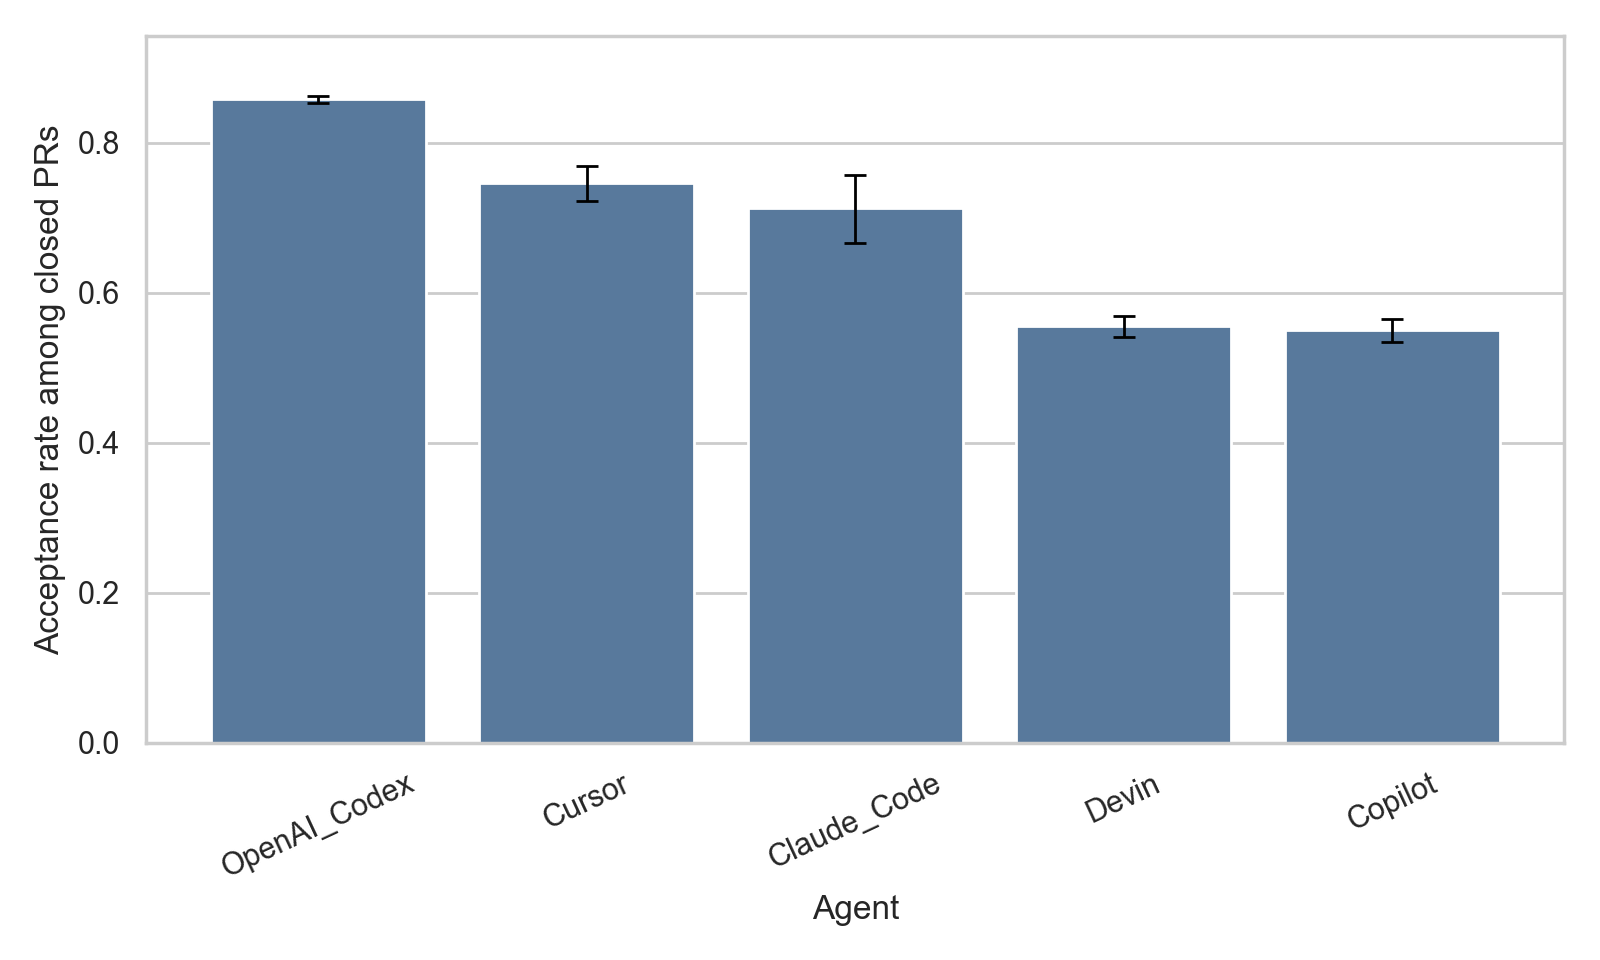
\includegraphics[width=\linewidth]{../figures/rq1_acceptance_by_agent.png}
  \caption{Acceptance rate by agent with confidence intervals.}
  \label{fig:rq1}
\end{figure}

The chi-square test indicates that merge outcome differs significantly across agents, $\chi^2 = 3179.35$, $df = 4$, $p < .001$. Figure~\ref{fig:rq1} visualizes these differences with confidence intervals.

These results indicate that agent identity is associated with acceptance. However, this association should not be interpreted as a direct ranking of agent quality. Different agents may be deployed in different repositories, for different tasks, and under different review expectations. RQ3 therefore models acceptance while controlling for project and change-level factors.

\subsection{RQ2: Review Turnaround Time by Agent}

Table~\ref{tab:rq2} reports review turnaround using time to first human response. Devin and OpenAI Codex have the shortest median human response times, while Claude Code has the longest median response time in this dataset.

\begin{table}[t]
  \caption{Time to first human response by agent.}
  \label{tab:rq2}
  \centering
  \begin{tabular}{lrrrr}
    \toprule
    Agent & PRs & Median & Mean & IQR \\
    \midrule
    Devin & 2,457 & 0.53 & 29.66 & 0.07--8.43 \\
    OpenAI Codex & 1,952 & 0.58 & 41.07 & 0.04--13.01 \\
    Copilot & 3,435 & 0.76 & 23.90 & 0.31--4.99 \\
    Cursor & 576 & 0.85 & 32.25 & 0.03--15.49 \\
    Claude Code & 221 & 1.09 & 50.66 & 0.09--13.95 \\
    \bottomrule
  \end{tabular}
\end{table}

\begin{figure}[t]
  \centering
  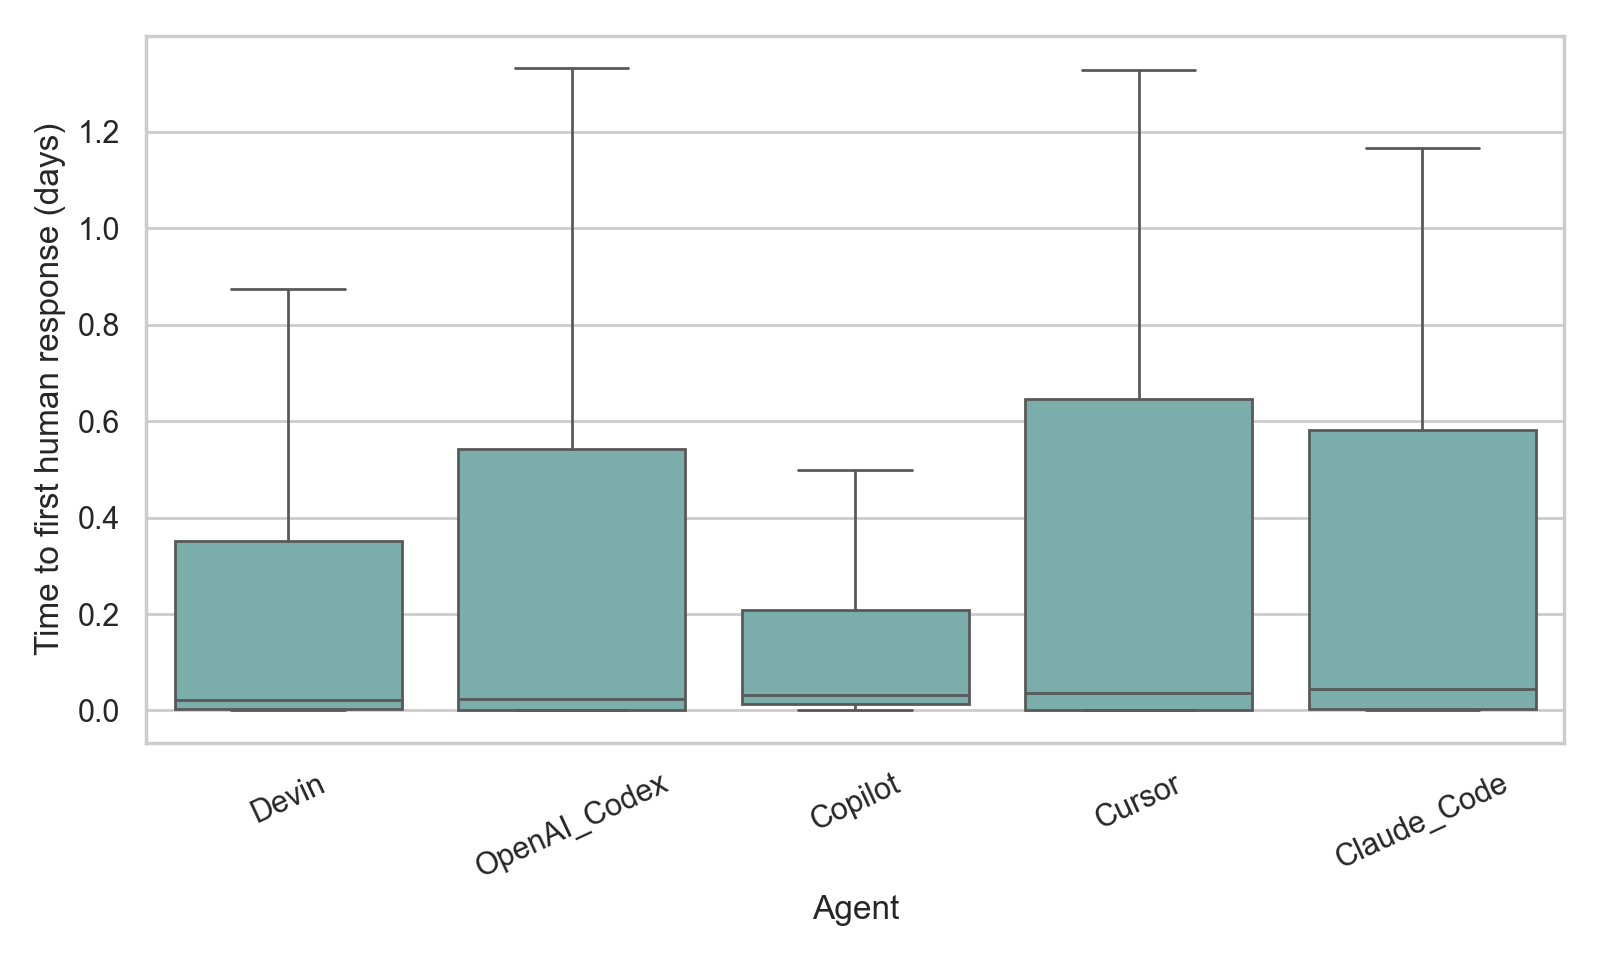
\includegraphics[width=\linewidth]{../figures/rq2_turnaround_by_agent.png}
  \caption{Median time to first human response by agent.}
  \label{fig:rq2}
\end{figure}

The Kruskal-Wallis test finds statistically significant differences in turnaround time across agents, $H = 89.70$, $p < .001$, based on 8,641 pull requests with a valid first human response time. Although the median response times are short for all agents, the means are much higher than the medians, indicating skewed distributions with some pull requests waiting much longer for human attention. These results suggest that AI-generated PRs can enter review workflows quickly, while review speed remains uneven and likely shaped by repository-specific practices.

\subsection{RQ3: Factors Associated with Acceptance}

The logistic regression model is fit on 31,284 closed pull requests. The model includes agent identity, repository stars and forks, language, PR size metrics, review/comment activity, repository AI PR volume, task type, touched file categories, and linked-issue status. The model has McFadden pseudo-$R^2 = 0.230$, with an overall likelihood-ratio $p < .001$.

\begin{table}[t]
  \caption{Selected logistic regression odds ratios for PR acceptance.}
  \label{tab:rq3}
  \centering
  \begin{tabular}{lrp{0.44\linewidth}}
    \toprule
    Factor & OR & Interpretation \\
    \midrule
    Review count & 7.70 & More review activity is associated with higher merge odds. \\
    Repository AI PR volume & 1.27 & Repositories with more AI PRs show higher acceptance odds. \\
    Comment count & 0.57 & More comments are associated with lower acceptance odds. \\
    Copilot vs baseline & 0.18 & Lower acceptance odds than the baseline agent category. \\
    Devin vs baseline & 0.21 & Lower acceptance odds than the baseline agent category. \\
    Churn & 0.88 & Larger changes are associated with lower acceptance odds. \\
    Forks & 0.80 & Higher fork count is associated with lower acceptance odds. \\
    Python language & 1.73 & Python projects show higher acceptance odds than the baseline language. \\
    HTML language & 2.90 & HTML projects show higher acceptance odds than the baseline language. \\
    Commit count & 1.34 & More commits are associated with higher acceptance odds. \\
    \bottomrule
  \end{tabular}
\end{table}

\begin{figure}[t]
  \centering
  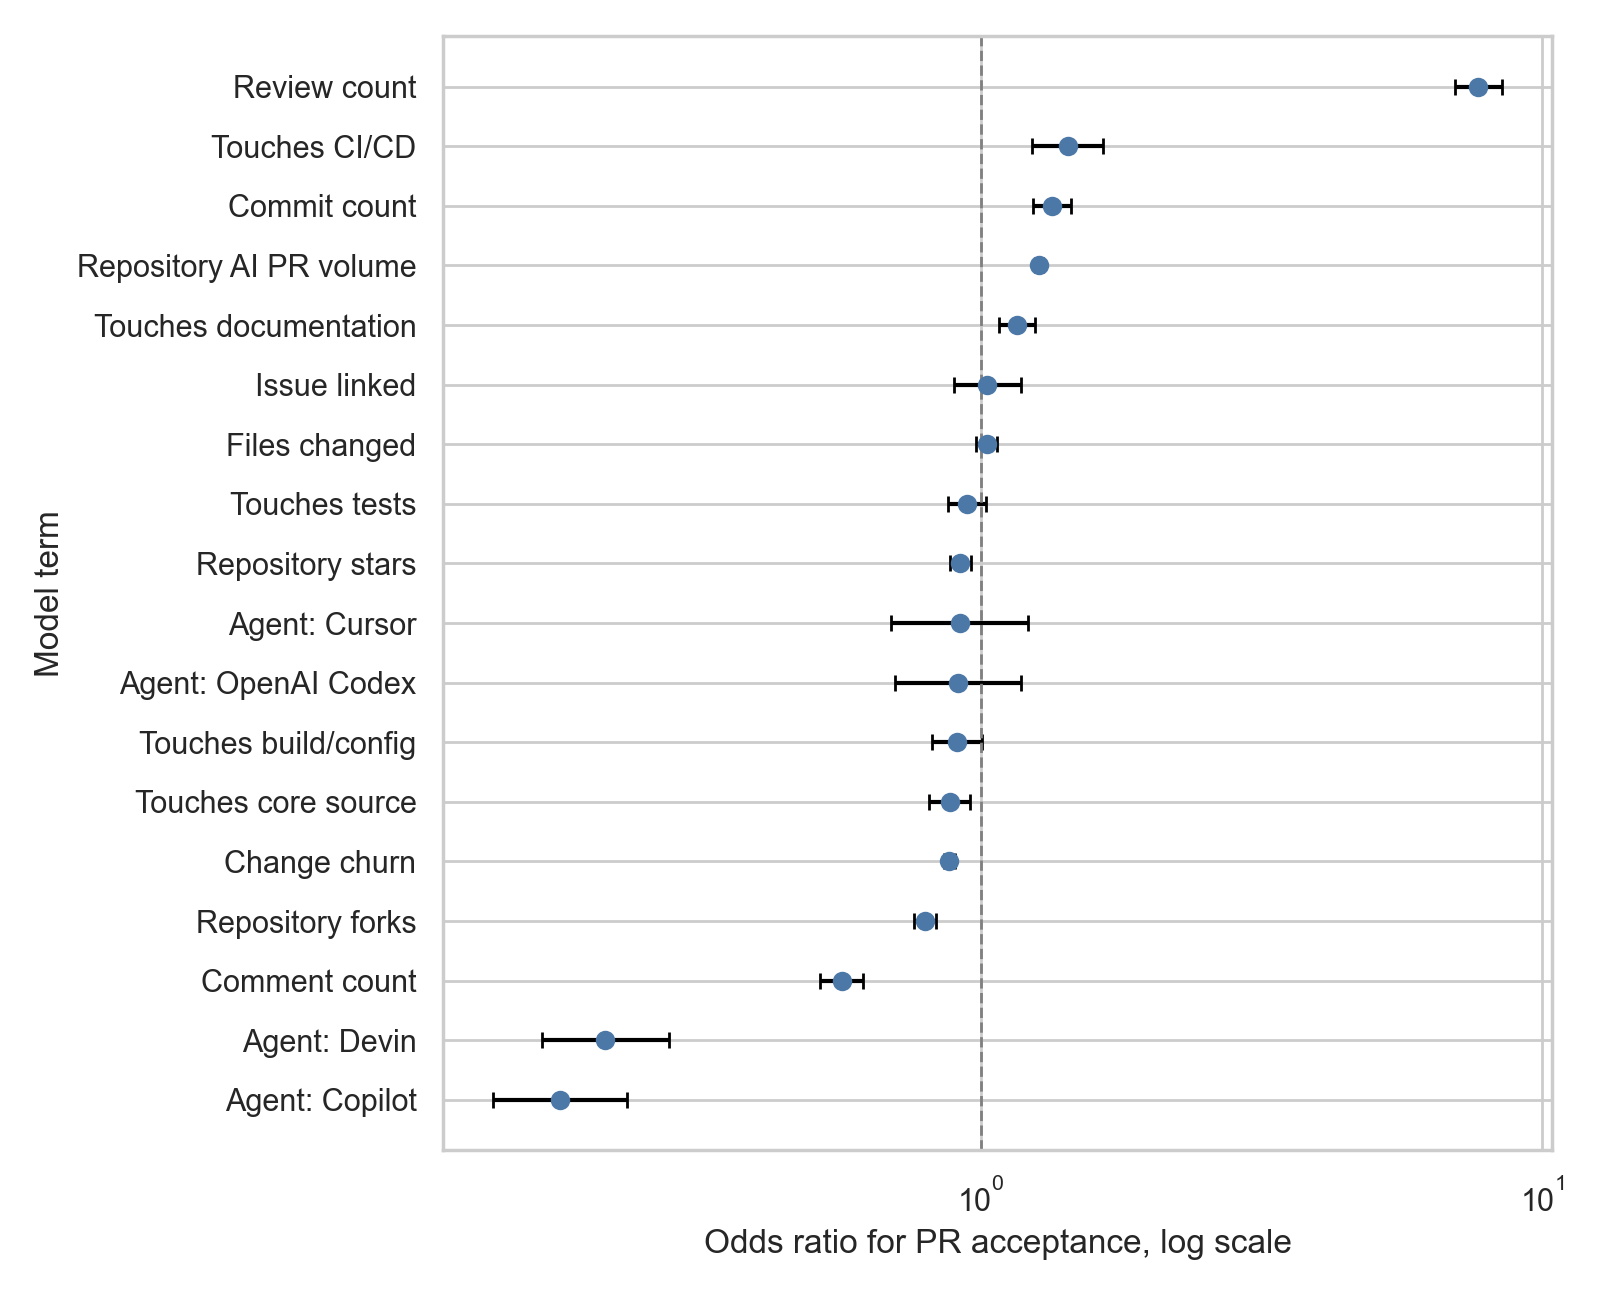
\includegraphics[width=\linewidth]{../figures/rq3_logistic_regression_odds_ratios.png}
  \caption{Selected odds ratios from the logistic regression model.}
  \label{fig:rq3}
\end{figure}

Table~\ref{tab:rq3} summarizes selected model terms with strong associations. The model indicates that acceptance is not explained by agent identity alone. Review activity is strongly associated with acceptance, while comment count has a negative association. One interpretation is that formal review activity may indicate progress toward integration, while longer comment discussions may reflect problems, uncertainty, or requested changes. Change size also matters: higher churn is associated with lower acceptance odds, consistent with the expectation that larger or riskier changes face more review friction.

Repository context is also associated with acceptance. Repository AI PR volume is positively associated with acceptance, suggesting that projects with more exposure to AI-generated pull requests may be more prepared to evaluate and integrate them. However, these results are observational and should be interpreted as associations rather than causal effects.

\subsection{RQ4-B: Core Source Code vs Peripheral Artifacts}

The additional research question examines whether AI-generated pull requests are more accepted when they modify peripheral artifacts rather than core source code. Table~\ref{tab:rq4scope} compares pull requests that touch core source files with pull requests that do not touch core source files.

\begin{table}[t]
  \caption{Acceptance by change scope.}
  \label{tab:rq4scope}
  \centering
  \begin{tabular}{lrrr}
    \toprule
    Change scope & Closed & Merged & Rate \\
    \midrule
    Peripheral/no core source & 8,959 & 7,214 & 80.5\% \\
    Touches core source & 22,325 & 16,800 & 75.3\% \\
    \bottomrule
  \end{tabular}
\end{table}

\begin{figure}[t]
  \centering
  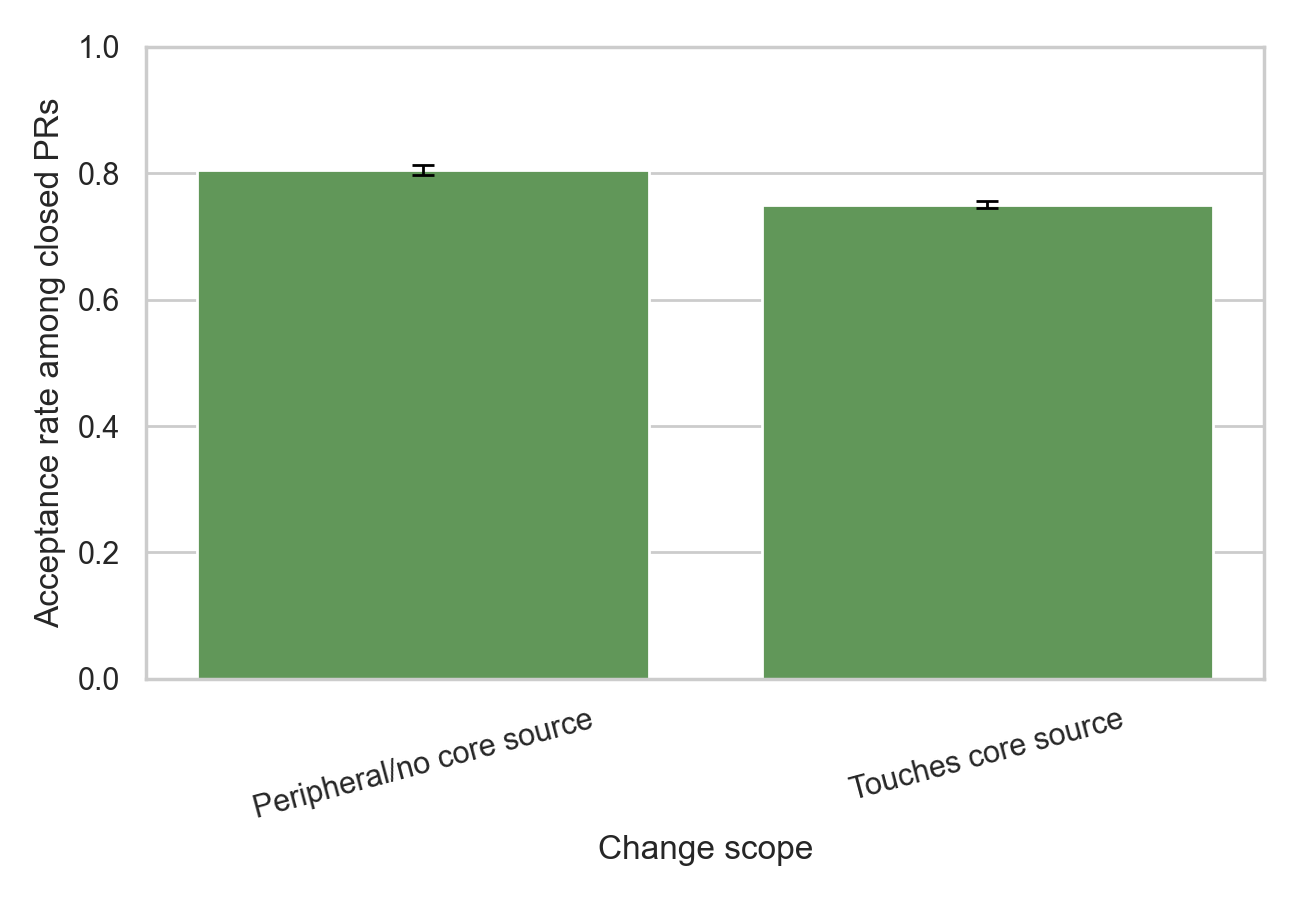
\includegraphics[width=\linewidth]{../figures/rq4b_acceptance_by_scope.png}
  \caption{Acceptance by core-source versus peripheral change scope.}
  \label{fig:rq4scope}
\end{figure}

The chi-square test indicates a significant difference between these groups, $\chi^2 = 99.26$, $df = 1$, $p < .001$. Table~\ref{tab:rq4cat} shows acceptance rates by file category. Because a pull request may touch multiple file categories, these category-level rows are not mutually exclusive; each row reports acceptance among closed pull requests that touched at least one file in that category.

\begin{table}[t]
  \caption{Acceptance by touched file category.}
  \label{tab:rq4cat}
  \centering
  \begin{tabular}{lrrr}
    \toprule
    File category & Closed & Merged & Rate \\
    \midrule
    Infrastructure & 80 & 65 & 81.3\% \\
    Documentation & 11,661 & 9,426 & 80.8\% \\
    CI/CD & 2,033 & 1,586 & 78.0\% \\
    Tests & 12,995 & 10,080 & 77.6\% \\
    Core source & 22,325 & 16,800 & 75.3\% \\
    Build/config & 4,113 & 2,761 & 67.1\% \\
    Other & 9,395 & 6,235 & 66.4\% \\
    Dependencies & 2,057 & 1,330 & 64.7\% \\
    \bottomrule
  \end{tabular}
\end{table}

\begin{figure}[t]
  \centering
  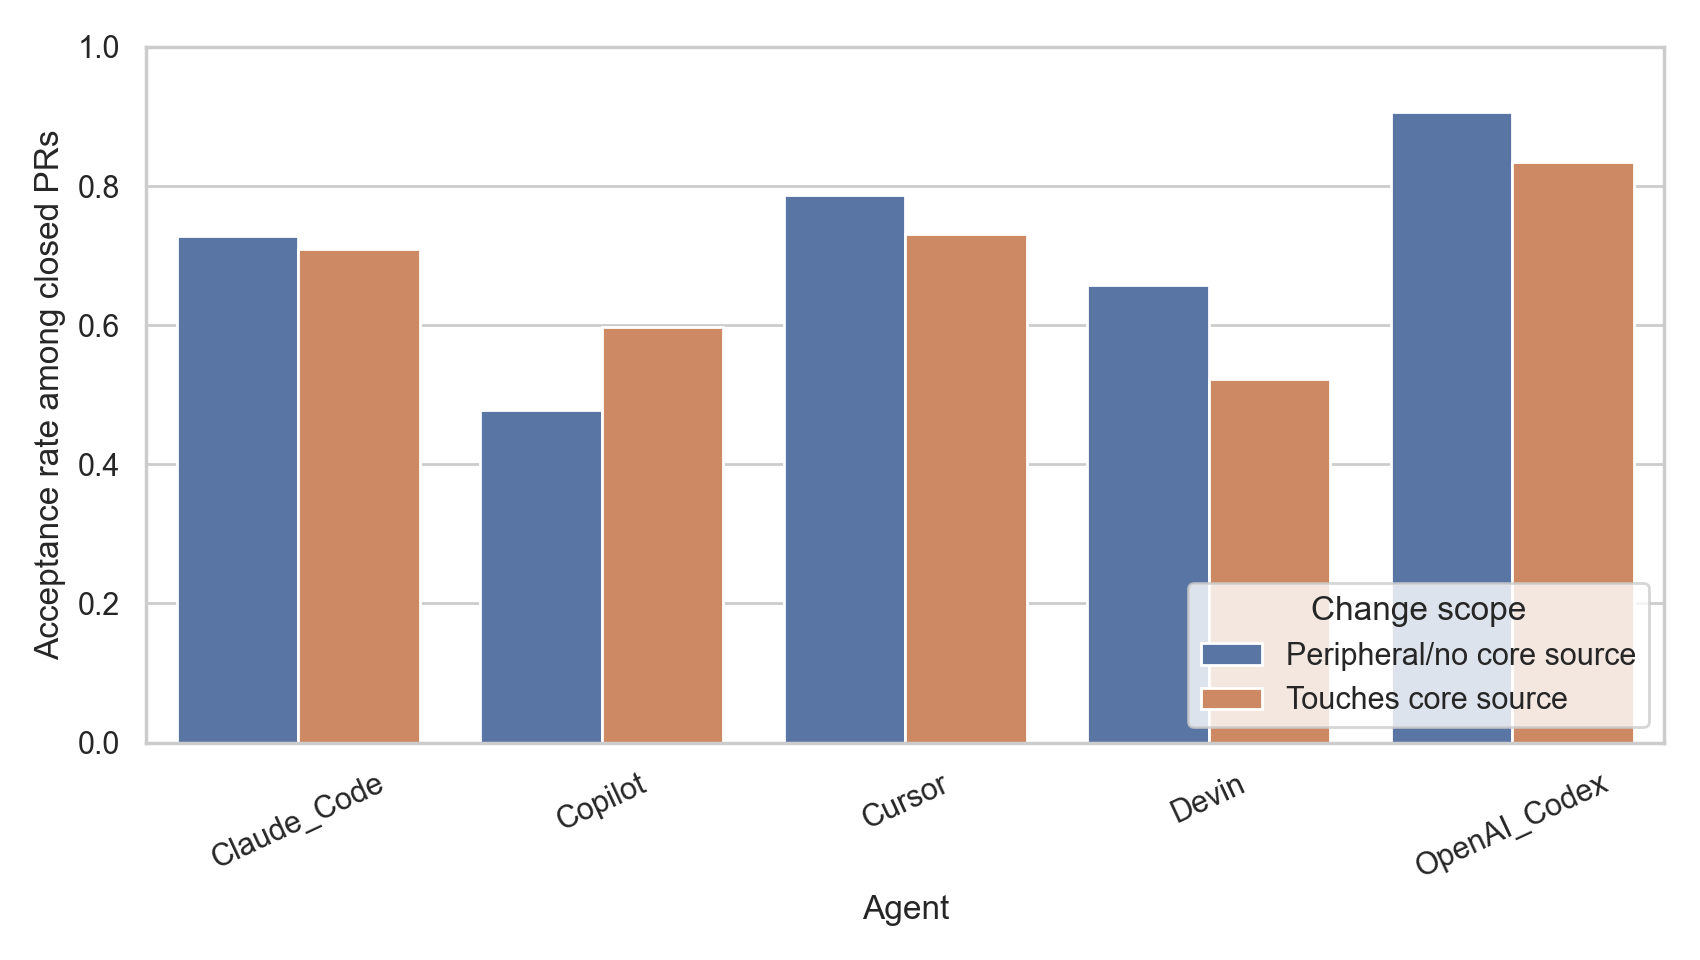
\includegraphics[width=\linewidth]{../figures/rq4b_acceptance_by_agent_and_scope.png}
  \caption{Acceptance by agent and change scope.}
  \label{fig:rq4agentscope}
\end{figure}

Overall, the results indicate that peripheral changes are accepted at a moderately higher rate than changes touching core source code. This pattern is consistent with the expectation that documentation, tests, and CI changes may be easier to review or lower risk than core logic changes. However, the practical difference is modest, and the by-agent breakdown shows that the pattern is not universal for every agent. For example, Copilot has higher acceptance for core-source changes than for peripheral changes in the processed results. This reinforces the broader finding that AI PR acceptance depends on the interaction between agent, task, repository, and change type.

\section{Discussion}

The findings characterize AI coding agents as meaningful but uneven participants in software evolution workflows. They are not accepted uniformly, and their success cannot be understood only by comparing agent names. Acceptance varies by agent, but also by review activity, repository context, programming language, change size, and file type.

From the perspective of intelligent tools for software evolution, the evidence is cautiously positive. Many AI-generated pull requests are merged, and median first-human-response times are short for the subset of PRs receiving human responses. This suggests that AI-generated contributions can fit into existing pull request workflows and receive timely attention.

At the same time, the results reveal limits in readiness. Larger changes are less likely to be accepted, and pull requests that generate more comment discussion are associated with lower acceptance odds. These patterns suggest that AI agents may currently be more reliable as assistants for bounded, reviewable changes than as autonomous producers of large or complex modifications.

The RQ4-B results also point to a practical role for AI agents. Peripheral artifacts such as documentation, tests, and CI/CD files are important for software evolution and maintenance. Higher acceptance in these areas suggests that AI agents may provide value by improving project support structures, reducing maintenance burden, and helping developers handle repetitive or lower-risk tasks.

Overall, the evidence suggests that AI coding agents are becoming viable software engineering teammates, while their readiness remains context-dependent. Effective use likely requires careful task selection, human review, repository-specific norms, and an understanding of where AI-generated changes are most trustworthy.

\section{Threats to Validity}

Construct validity is limited by the operational definitions used in the analysis. Acceptance is measured using merge status, which is a practical outcome but not a direct measure of code quality, maintainability, or developer satisfaction. A merged pull request may still contain issues, and an unmerged pull request may be valuable but rejected for reasons unrelated to quality.

Review turnaround is measured as the time to first human review or comment. This captures visible GitHub activity, but it may miss discussion that occurred outside the platform or in other communication channels. It also measures first response rather than full review completion.

The file-category classification is heuristic. It uses file paths and extensions to infer whether a file is core source code, documentation, tests, CI/CD, configuration, dependencies, infrastructure, or other. This approach is scalable but imperfect; some files may be misclassified, especially in repositories with unusual layouts.

Internal validity is limited because the regression model shows association, not causation. For example, more reviews are associated with higher acceptance, but the model cannot prove that reviews cause acceptance. Review activity may instead be a signal that maintainers were already interested in merging the pull request.

External validity is limited by the dataset. The AIDev dataset may not represent all open-source projects, all industrial settings, or all AI coding agents. Results may differ for private repositories, different review cultures, newer agent versions, or projects with different governance structures.

Finally, some results may be affected by missing data or dataset-specific collection choices. Pull requests without visible reviews or comments are excluded from the RQ2 turnaround-time calculation, which means RQ2 describes PRs with observed human responses rather than all AI-generated PRs.

\section{Conclusion}

This paper analyzed AI-generated pull requests from the AIDev dataset to examine how AI coding agents behave as tools for software evolution. The results show significant differences in acceptance rates across agents, significant differences in first human response time, and strong associations between acceptance and project/change factors. The additional analysis indicates that pull requests not touching core source code have moderately higher acceptance rates overall than pull requests touching core source code.

These findings suggest that AI coding agents are not simply interchangeable code generators. Their success depends on the surrounding software engineering context, including repository practices, task type, review activity, and the risk level of the change. AI agents appear promising as software engineering teammates, especially for well-scoped and lower-risk contributions, but they still require human review and careful integration into project workflows.

\section*{AI Usage Acknowledgement}

The authors used ChatGPT/Codex to support analysis planning, repository inspection, requirement interpretation, and manuscript drafting. The reported analyses, results, and interpretations remain the responsibility of the authors.

\bibliographystyle{ACM-Reference-Format}
\bibliography{references}

\end{document}
